% Generated by ArticleSignalDiagrams. Opaque vector fills only.
\documentclass[10pt,tikz,border=5pt]{standalone}
\usepackage{lmodern}
\usetikzlibrary{fit}
\begin{document}
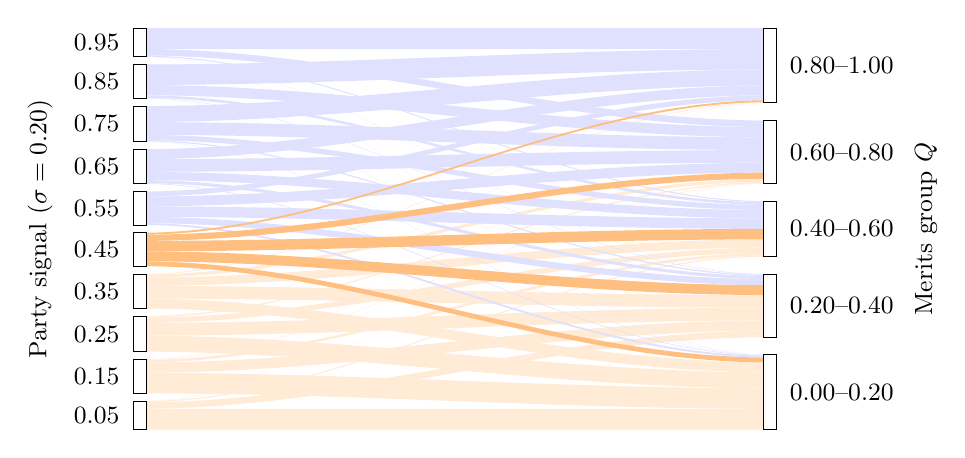
\begin{tikzpicture}[x=1cm,y=1cm,font=\small]\path[fill=orange!16!white,draw=none] (3.3,-5.1) .. controls (6,-5.1) and (8.6,-5.1) .. (11.3,-5.1) -- (11.3,-4.834961) .. controls (8.6,-4.834961) and (6,-4.834961) .. (3.3,-4.834961) -- cycle;
\path[fill=orange!16!white,draw=none] (3.3,-4.834961) .. controls (6,-4.834961) and (8.6,-3.925338) .. (11.3,-3.925338) -- (11.3,-3.842552) .. controls (8.6,-3.842552) and (6,-4.752175) .. (3.3,-4.752175) -- cycle;
\path[fill=orange!16!white,draw=none] (3.3,-4.752175) .. controls (6,-4.752175) and (8.6,-2.901408) .. (11.3,-2.901408) -- (11.3,-2.888177) .. controls (8.6,-2.888177) and (6,-4.738944) .. (3.3,-4.738944) -- cycle;
\path[fill=orange!16!white,draw=none] (3.3,-4.738944) .. controls (6,-4.738944) and (8.6,-1.973592) .. (11.3,-1.973592) -- (11.3,-1.972415) .. controls (8.6,-1.972415) and (6,-4.737767) .. (3.3,-4.737767) -- cycle;
\path[fill=orange!16!white,draw=none] (3.3,-4.737767) .. controls (6,-4.737767) and (8.6,-0.949662) .. (11.3,-0.949662) -- (11.3,-0.949608) .. controls (8.6,-0.949608) and (6,-4.737713) .. (3.3,-4.737713) -- cycle;
\path[fill=orange!16!white,draw=none] (3.3,-4.637713) .. controls (6,-4.637713) and (8.6,-4.834961) .. (11.3,-4.834961) -- (11.3,-4.574794) .. controls (8.6,-4.574794) and (6,-4.377546) .. (3.3,-4.377546) -- cycle;
\path[fill=orange!16!white,draw=none] (3.3,-4.377546) .. controls (6,-4.377546) and (8.6,-3.842552) .. (11.3,-3.842552) -- (11.3,-3.712672) .. controls (8.6,-3.712672) and (6,-4.247666) .. (3.3,-4.247666) -- cycle;
\path[fill=orange!16!white,draw=none] (3.3,-4.247666) .. controls (6,-4.247666) and (8.6,-2.888177) .. (11.3,-2.888177) -- (11.3,-2.85484) .. controls (8.6,-2.85484) and (6,-4.214328) .. (3.3,-4.214328) -- cycle;
\path[fill=orange!16!white,draw=none] (3.3,-4.214328) .. controls (6,-4.214328) and (8.6,-1.972415) .. (11.3,-1.972415) -- (11.3,-1.967642) .. controls (8.6,-1.967642) and (6,-4.209555) .. (3.3,-4.209555) -- cycle;
\path[fill=orange!16!white,draw=none] (3.3,-4.209555) .. controls (6,-4.209555) and (8.6,-0.949608) .. (11.3,-0.949608) -- (11.3,-0.949252) .. controls (8.6,-0.949252) and (6,-4.209199) .. (3.3,-4.209199) -- cycle;
\path[fill=orange!16!white,draw=none] (3.3,-4.109199) .. controls (6,-4.109199) and (8.6,-4.574794) .. (11.3,-4.574794) -- (11.3,-4.371886) .. controls (8.6,-4.371886) and (6,-3.906291) .. (3.3,-3.906291) -- cycle;
\path[fill=orange!16!white,draw=none] (3.3,-3.906291) .. controls (6,-3.906291) and (8.6,-3.712672) .. (11.3,-3.712672) -- (11.3,-3.55093) .. controls (8.6,-3.55093) and (6,-3.74455) .. (3.3,-3.74455) -- cycle;
\path[fill=orange!16!white,draw=none] (3.3,-3.74455) .. controls (6,-3.74455) and (8.6,-2.85484) .. (11.3,-2.85484) -- (11.3,-2.788266) .. controls (8.6,-2.788266) and (6,-3.677976) .. (3.3,-3.677976) -- cycle;
\path[fill=orange!16!white,draw=none] (3.3,-3.677976) .. controls (6,-3.677976) and (8.6,-1.967642) .. (11.3,-1.967642) -- (11.3,-1.952322) .. controls (8.6,-1.952322) and (6,-3.662657) .. (3.3,-3.662657) -- cycle;
\path[fill=orange!16!white,draw=none] (3.3,-3.662657) .. controls (6,-3.662657) and (8.6,-0.949252) .. (11.3,-0.949252) -- (11.3,-0.947416) .. controls (8.6,-0.947416) and (6,-3.660821) .. (3.3,-3.660821) -- cycle;
\path[fill=orange!16!white,draw=none] (3.3,-3.560821) .. controls (6,-3.560821) and (8.6,-4.371886) .. (11.3,-4.371886) -- (11.3,-4.246143) .. controls (8.6,-4.246143) and (6,-3.435078) .. (3.3,-3.435078) -- cycle;
\path[fill=orange!16!white,draw=none] (3.3,-3.435078) .. controls (6,-3.435078) and (8.6,-3.55093) .. (11.3,-3.55093) -- (11.3,-3.390931) .. controls (8.6,-3.390931) and (6,-3.27508) .. (3.3,-3.27508) -- cycle;
\path[fill=orange!16!white,draw=none] (3.3,-3.27508) .. controls (6,-3.27508) and (8.6,-2.788266) .. (11.3,-2.788266) -- (11.3,-2.68277) .. controls (8.6,-2.68277) and (6,-3.169584) .. (3.3,-3.169584) -- cycle;
\path[fill=orange!16!white,draw=none] (3.3,-3.169584) .. controls (6,-3.169584) and (8.6,-1.952322) .. (11.3,-1.952322) -- (11.3,-1.913376) .. controls (8.6,-1.913376) and (6,-3.130638) .. (3.3,-3.130638) -- cycle;
\path[fill=orange!16!white,draw=none] (3.3,-3.130638) .. controls (6,-3.130638) and (8.6,-0.947416) .. (11.3,-0.947416) -- (11.3,-0.939929) .. controls (8.6,-0.939929) and (6,-3.12315) .. (3.3,-3.12315) -- cycle;
\path[fill=blue!12!white,draw=none] (3.3,-2.5) .. controls (6,-2.5) and (8.6,-4.18425) .. (11.3,-4.18425) -- (11.3,-4.160071) .. controls (8.6,-4.160071) and (6,-2.475821) .. (3.3,-2.475821) -- cycle;
\path[fill=blue!12!white,draw=none] (3.3,-2.475821) .. controls (6,-2.475821) and (8.6,-3.265165) .. (11.3,-3.265165) -- (11.3,-3.186624) .. controls (8.6,-3.186624) and (6,-2.39728) .. (3.3,-2.39728) -- cycle;
\path[fill=blue!12!white,draw=none] (3.3,-2.39728) .. controls (6,-2.39728) and (8.6,-2.55) .. (11.3,-2.55) -- (11.3,-2.41723) .. controls (8.6,-2.41723) and (6,-2.26451) .. (3.3,-2.26451) -- cycle;
\path[fill=blue!12!white,draw=none] (3.3,-2.26451) .. controls (6,-2.26451) and (8.6,-1.834835) .. (11.3,-1.834835) -- (11.3,-1.709069) .. controls (8.6,-1.709069) and (6,-2.138744) .. (3.3,-2.138744) -- cycle;
\path[fill=blue!12!white,draw=none] (3.3,-2.138744) .. controls (6,-2.138744) and (8.6,-0.91575) .. (11.3,-0.91575) -- (11.3,-0.853857) .. controls (8.6,-0.853857) and (6,-2.07685) .. (3.3,-2.07685) -- cycle;
\path[fill=blue!12!white,draw=none] (3.3,-1.97685) .. controls (6,-1.97685) and (8.6,-4.160071) .. (11.3,-4.160071) -- (11.3,-4.152584) .. controls (8.6,-4.152584) and (6,-1.969362) .. (3.3,-1.969362) -- cycle;
\path[fill=blue!12!white,draw=none] (3.3,-1.969362) .. controls (6,-1.969362) and (8.6,-3.186624) .. (11.3,-3.186624) -- (11.3,-3.147678) .. controls (8.6,-3.147678) and (6,-1.930416) .. (3.3,-1.930416) -- cycle;
\path[fill=blue!12!white,draw=none] (3.3,-1.930416) .. controls (6,-1.930416) and (8.6,-2.41723) .. (11.3,-2.41723) -- (11.3,-2.311734) .. controls (8.6,-2.311734) and (6,-1.82492) .. (3.3,-1.82492) -- cycle;
\path[fill=blue!12!white,draw=none] (3.3,-1.82492) .. controls (6,-1.82492) and (8.6,-1.709069) .. (11.3,-1.709069) -- (11.3,-1.54907) .. controls (8.6,-1.54907) and (6,-1.664922) .. (3.3,-1.664922) -- cycle;
\path[fill=blue!12!white,draw=none] (3.3,-1.664922) .. controls (6,-1.664922) and (8.6,-0.853857) .. (11.3,-0.853857) -- (11.3,-0.728114) .. controls (8.6,-0.728114) and (6,-1.539179) .. (3.3,-1.539179) -- cycle;
\path[fill=blue!12!white,draw=none] (3.3,-1.439179) .. controls (6,-1.439179) and (8.6,-4.152584) .. (11.3,-4.152584) -- (11.3,-4.150748) .. controls (8.6,-4.150748) and (6,-1.437343) .. (3.3,-1.437343) -- cycle;
\path[fill=blue!12!white,draw=none] (3.3,-1.437343) .. controls (6,-1.437343) and (8.6,-3.147678) .. (11.3,-3.147678) -- (11.3,-3.132358) .. controls (8.6,-3.132358) and (6,-1.422024) .. (3.3,-1.422024) -- cycle;
\path[fill=blue!12!white,draw=none] (3.3,-1.422024) .. controls (6,-1.422024) and (8.6,-2.311734) .. (11.3,-2.311734) -- (11.3,-2.24516) .. controls (8.6,-2.24516) and (6,-1.35545) .. (3.3,-1.35545) -- cycle;
\path[fill=blue!12!white,draw=none] (3.3,-1.35545) .. controls (6,-1.35545) and (8.6,-1.54907) .. (11.3,-1.54907) -- (11.3,-1.387328) .. controls (8.6,-1.387328) and (6,-1.193709) .. (3.3,-1.193709) -- cycle;
\path[fill=blue!12!white,draw=none] (3.3,-1.193709) .. controls (6,-1.193709) and (8.6,-0.728114) .. (11.3,-0.728114) -- (11.3,-0.525206) .. controls (8.6,-0.525206) and (6,-0.990801) .. (3.3,-0.990801) -- cycle;
\path[fill=blue!12!white,draw=none] (3.3,-0.890801) .. controls (6,-0.890801) and (8.6,-4.150748) .. (11.3,-4.150748) -- (11.3,-4.150392) .. controls (8.6,-4.150392) and (6,-0.890445) .. (3.3,-0.890445) -- cycle;
\path[fill=blue!12!white,draw=none] (3.3,-0.890445) .. controls (6,-0.890445) and (8.6,-3.132358) .. (11.3,-3.132358) -- (11.3,-3.127585) .. controls (8.6,-3.127585) and (6,-0.885672) .. (3.3,-0.885672) -- cycle;
\path[fill=blue!12!white,draw=none] (3.3,-0.885672) .. controls (6,-0.885672) and (8.6,-2.24516) .. (11.3,-2.24516) -- (11.3,-2.211823) .. controls (8.6,-2.211823) and (6,-0.852334) .. (3.3,-0.852334) -- cycle;
\path[fill=blue!12!white,draw=none] (3.3,-0.852334) .. controls (6,-0.852334) and (8.6,-1.387328) .. (11.3,-1.387328) -- (11.3,-1.257448) .. controls (8.6,-1.257448) and (6,-0.722454) .. (3.3,-0.722454) -- cycle;
\path[fill=blue!12!white,draw=none] (3.3,-0.722454) .. controls (6,-0.722454) and (8.6,-0.525206) .. (11.3,-0.525206) -- (11.3,-0.265039) .. controls (8.6,-0.265039) and (6,-0.462287) .. (3.3,-0.462287) -- cycle;
\path[fill=blue!12!white,draw=none] (3.3,-0.362287) .. controls (6,-0.362287) and (8.6,-4.150392) .. (11.3,-4.150392) -- (11.3,-4.150338) .. controls (8.6,-4.150338) and (6,-0.362233) .. (3.3,-0.362233) -- cycle;
\path[fill=blue!12!white,draw=none] (3.3,-0.362233) .. controls (6,-0.362233) and (8.6,-3.127585) .. (11.3,-3.127585) -- (11.3,-3.126408) .. controls (8.6,-3.126408) and (6,-0.361056) .. (3.3,-0.361056) -- cycle;
\path[fill=blue!12!white,draw=none] (3.3,-0.361056) .. controls (6,-0.361056) and (8.6,-2.211823) .. (11.3,-2.211823) -- (11.3,-2.198592) .. controls (8.6,-2.198592) and (6,-0.347825) .. (3.3,-0.347825) -- cycle;
\path[fill=blue!12!white,draw=none] (3.3,-0.347825) .. controls (6,-0.347825) and (8.6,-1.257448) .. (11.3,-1.257448) -- (11.3,-1.174662) .. controls (8.6,-1.174662) and (6,-0.265039) .. (3.3,-0.265039) -- cycle;
\path[fill=blue!12!white,draw=none] (3.3,-0.265039) .. controls (6,-0.265039) and (8.6,-0.265039) .. (11.3,-0.265039) -- (11.3,0) .. controls (8.6,0) and (6,0) .. (3.3,0) -- cycle;
\path[fill=orange!50!white,draw=none] (3.3,-3.02315) .. controls (6,-3.02315) and (8.6,-4.246143) .. (11.3,-4.246143) -- (11.3,-4.18425) .. controls (8.6,-4.18425) and (6,-2.961256) .. (3.3,-2.961256) -- cycle;
\path[fill=orange!50!white,draw=none] (3.3,-2.961256) .. controls (6,-2.961256) and (8.6,-3.390931) .. (11.3,-3.390931) -- (11.3,-3.265165) .. controls (8.6,-3.265165) and (6,-2.83549) .. (3.3,-2.83549) -- cycle;
\path[fill=orange!50!white,draw=none] (3.3,-2.83549) .. controls (6,-2.83549) and (8.6,-2.68277) .. (11.3,-2.68277) -- (11.3,-2.55) .. controls (8.6,-2.55) and (6,-2.70272) .. (3.3,-2.70272) -- cycle;
\path[fill=orange!50!white,draw=none] (3.3,-2.70272) .. controls (6,-2.70272) and (8.6,-1.913376) .. (11.3,-1.913376) -- (11.3,-1.834835) .. controls (8.6,-1.834835) and (6,-2.624179) .. (3.3,-2.624179) -- cycle;
\path[fill=orange!50!white,draw=none] (3.3,-2.624179) .. controls (6,-2.624179) and (8.6,-0.939929) .. (11.3,-0.939929) -- (11.3,-0.91575) .. controls (8.6,-0.91575) and (6,-2.6) .. (3.3,-2.6) -- cycle;
\coordinate (axis-midline-0) at (0,-2.55);
\path[fill=white,draw=black,line width=0.3pt] (3.22,-5.1) rectangle (3.38,-4.737713);
\node[anchor=east,fill=white,inner sep=2pt] (bucket-0-0-0) at (3.12,-4.918856) {0.05};
\path[fill=white,draw=black,line width=0.3pt] (3.22,-4.637713) rectangle (3.38,-4.209199);
\node[anchor=east,fill=white,inner sep=2pt] (bucket-0-0-1) at (3.12,-4.423456) {0.15};
\path[fill=white,draw=black,line width=0.3pt] (3.22,-4.109199) rectangle (3.38,-3.660821);
\node[anchor=east,fill=white,inner sep=2pt] (bucket-0-0-2) at (3.12,-3.88501) {0.25};
\path[fill=white,draw=black,line width=0.3pt] (3.22,-3.560821) rectangle (3.38,-3.12315);
\node[anchor=east,fill=white,inner sep=2pt] (bucket-0-0-3) at (3.12,-3.341986) {0.35};
\path[fill=white,draw=black,line width=0.3pt] (3.22,-3.02315) rectangle (3.38,-2.6);
\node[anchor=east,fill=white,inner sep=2pt] (bucket-0-0-4) at (3.12,-2.811575) {0.45};
\path[fill=white,draw=black,line width=0.3pt] (3.22,-2.5) rectangle (3.38,-2.07685);
\node[anchor=east,fill=white,inner sep=2pt] (bucket-0-0-5) at (3.12,-2.288425) {0.55};
\path[fill=white,draw=black,line width=0.3pt] (3.22,-1.97685) rectangle (3.38,-1.539179);
\node[anchor=east,fill=white,inner sep=2pt] (bucket-0-0-6) at (3.12,-1.758014) {0.65};
\path[fill=white,draw=black,line width=0.3pt] (3.22,-1.439179) rectangle (3.38,-0.990801);
\node[anchor=east,fill=white,inner sep=2pt] (bucket-0-0-7) at (3.12,-1.21499) {0.75};
\path[fill=white,draw=black,line width=0.3pt] (3.22,-0.890801) rectangle (3.38,-0.462287);
\node[anchor=east,fill=white,inner sep=2pt] (bucket-0-0-8) at (3.12,-0.676544) {0.85};
\path[fill=white,draw=black,line width=0.3pt] (3.22,-0.362287) rectangle (3.38,0);
\node[anchor=east,fill=white,inner sep=2pt] (bucket-0-0-9) at (3.12,-0.181144) {0.95};
\node[fit=(bucket-0-0-0) (bucket-0-0-1) (bucket-0-0-2) (bucket-0-0-3) (bucket-0-0-4) (bucket-0-0-5) (bucket-0-0-6) (bucket-0-0-7) (bucket-0-0-8) (bucket-0-0-9),inner sep=0pt] (source-labels-0) {};
\coordinate (axis-title-0-0) at (source-labels-0.west |- axis-midline-0);
\node[rotate=90,anchor=south,inner sep=0pt] at ([xshift=-0.18cm]axis-title-0-0) {Party signal ($\sigma=0.20$)};
\path[fill=white,draw=black,line width=0.3pt] (11.22,-5.1) rectangle (11.38,-4.150338);
\node[anchor=west,fill=white,inner sep=2pt] (bucket-0-1-0) at (11.48,-4.625169) {0.00--0.20};
\path[fill=white,draw=black,line width=0.3pt] (11.22,-3.925338) rectangle (11.38,-3.126408);
\node[anchor=west,fill=white,inner sep=2pt] (bucket-0-1-1) at (11.48,-3.525873) {0.20--0.40};
\path[fill=white,draw=black,line width=0.3pt] (11.22,-2.901408) rectangle (11.38,-2.198592);
\node[anchor=west,fill=white,inner sep=2pt] (bucket-0-1-2) at (11.48,-2.55) {0.40--0.60};
\path[fill=white,draw=black,line width=0.3pt] (11.22,-1.973592) rectangle (11.38,-1.174662);
\node[anchor=west,fill=white,inner sep=2pt] (bucket-0-1-3) at (11.48,-1.574127) {0.60--0.80};
\path[fill=white,draw=black,line width=0.3pt] (11.22,-0.949662) rectangle (11.38,0);
\node[anchor=west,fill=white,inner sep=2pt] (bucket-0-1-4) at (11.48,-0.474831) {0.80--1.00};
\node[fit=(bucket-0-1-0) (bucket-0-1-1) (bucket-0-1-2) (bucket-0-1-3) (bucket-0-1-4),inner sep=0pt] (destination-labels-0) {};
\coordinate (axis-title-0-1) at (destination-labels-0.east |- axis-midline-0);
\node[rotate=90,anchor=north,inner sep=0pt] at ([xshift=0.18cm]axis-title-0-1) {Merits group $Q$};
\end{tikzpicture}
\end{document}

